

Über den Menüpunkt \glqq Cleanup\grqq{} gelangt der Nutzer zur zentralen Funktionalität der Anwendung: dem Löschen temporärer und überflüssiger Dateien. In diesem Bereich kann der Benutzer gezielt konfigurieren, welche Dateien gelöscht werden sollen und in welchem Ordner die Bereinigung erfolgen soll.

\begin{itemize}
    \item \textbf{Pfad des Ordners:} Angabe des zu bereinigenden Verzeichnisses.
    \item \textbf{Älter als (Tage):} Legt fest, wie alt Dateien mindestens sein müssen, um als löschwürdig zu gelten.
    \item \textbf{Dateimuster:} Ermöglicht die Einschränkung der Löschung auf bestimmte Dateitypen (z.\,B. \texttt{*.tmp, *.log}); auch einzelne Dateien können gezielt gefiltert werden.
\end{itemize}

Der Pfad des Ordners muss nicht manuell eingegeben werden, sondern kann auch über den Button links neben dem Eingabefeld ausgewählt werden. Hierbei öffnet sich ein Dialogfenster (Windows-Explorer), über das der gewünschte Zielpfad bequem ausgewählt werden kann.

\vspace{1em}
Dem Benutzer stehen drei Buttons zur Verfügung:

\begin{itemize}
    \item \textbf{Clean Up:} Startet die Standard-Bereinigung gemäß der angegebenen Kriterien.
    \item \textbf{Junk Files löschen:} Sucht gezielt nach typischen temporären oder nutzlosen Dateien und entfernt diese.
    \item \textbf{Duplikate löschen:} Erkennt und entfernt doppelt vorhandene Dateien im gewählten Verzeichnis. Wichtig ist, dass nur die Duplikate gelöscht werden – die zuerst gefundene Originaldatei bleibt erhalten.
\end{itemize}

\vspace{1em}
Darunter befindet sich der Bereich \textbf{Scheduler-Einstellungen}. Hier kann der Benutzer ein automatisches Cleanup-Intervall (in Minuten) festlegen. Die Anwendung führt dann selbstständig in regelmäßigen Abständen eine Bereinigung durch.

\begin{itemize}
    \item \textbf{Scheduler starten:} Aktiviert die automatische Bereinigung.
    \item \textbf{Scheduler stoppen:} Deaktiviert den geplanten Bereinigungsprozess.
\end{itemize}

Eine Statusanzeige informiert den Nutzer darüber, wann die nächste automatische Bereinigung stattfinden wird oder ob der Vorgang bereits abgeschlossen ist.

\begin{figure}[H]
    \centering
    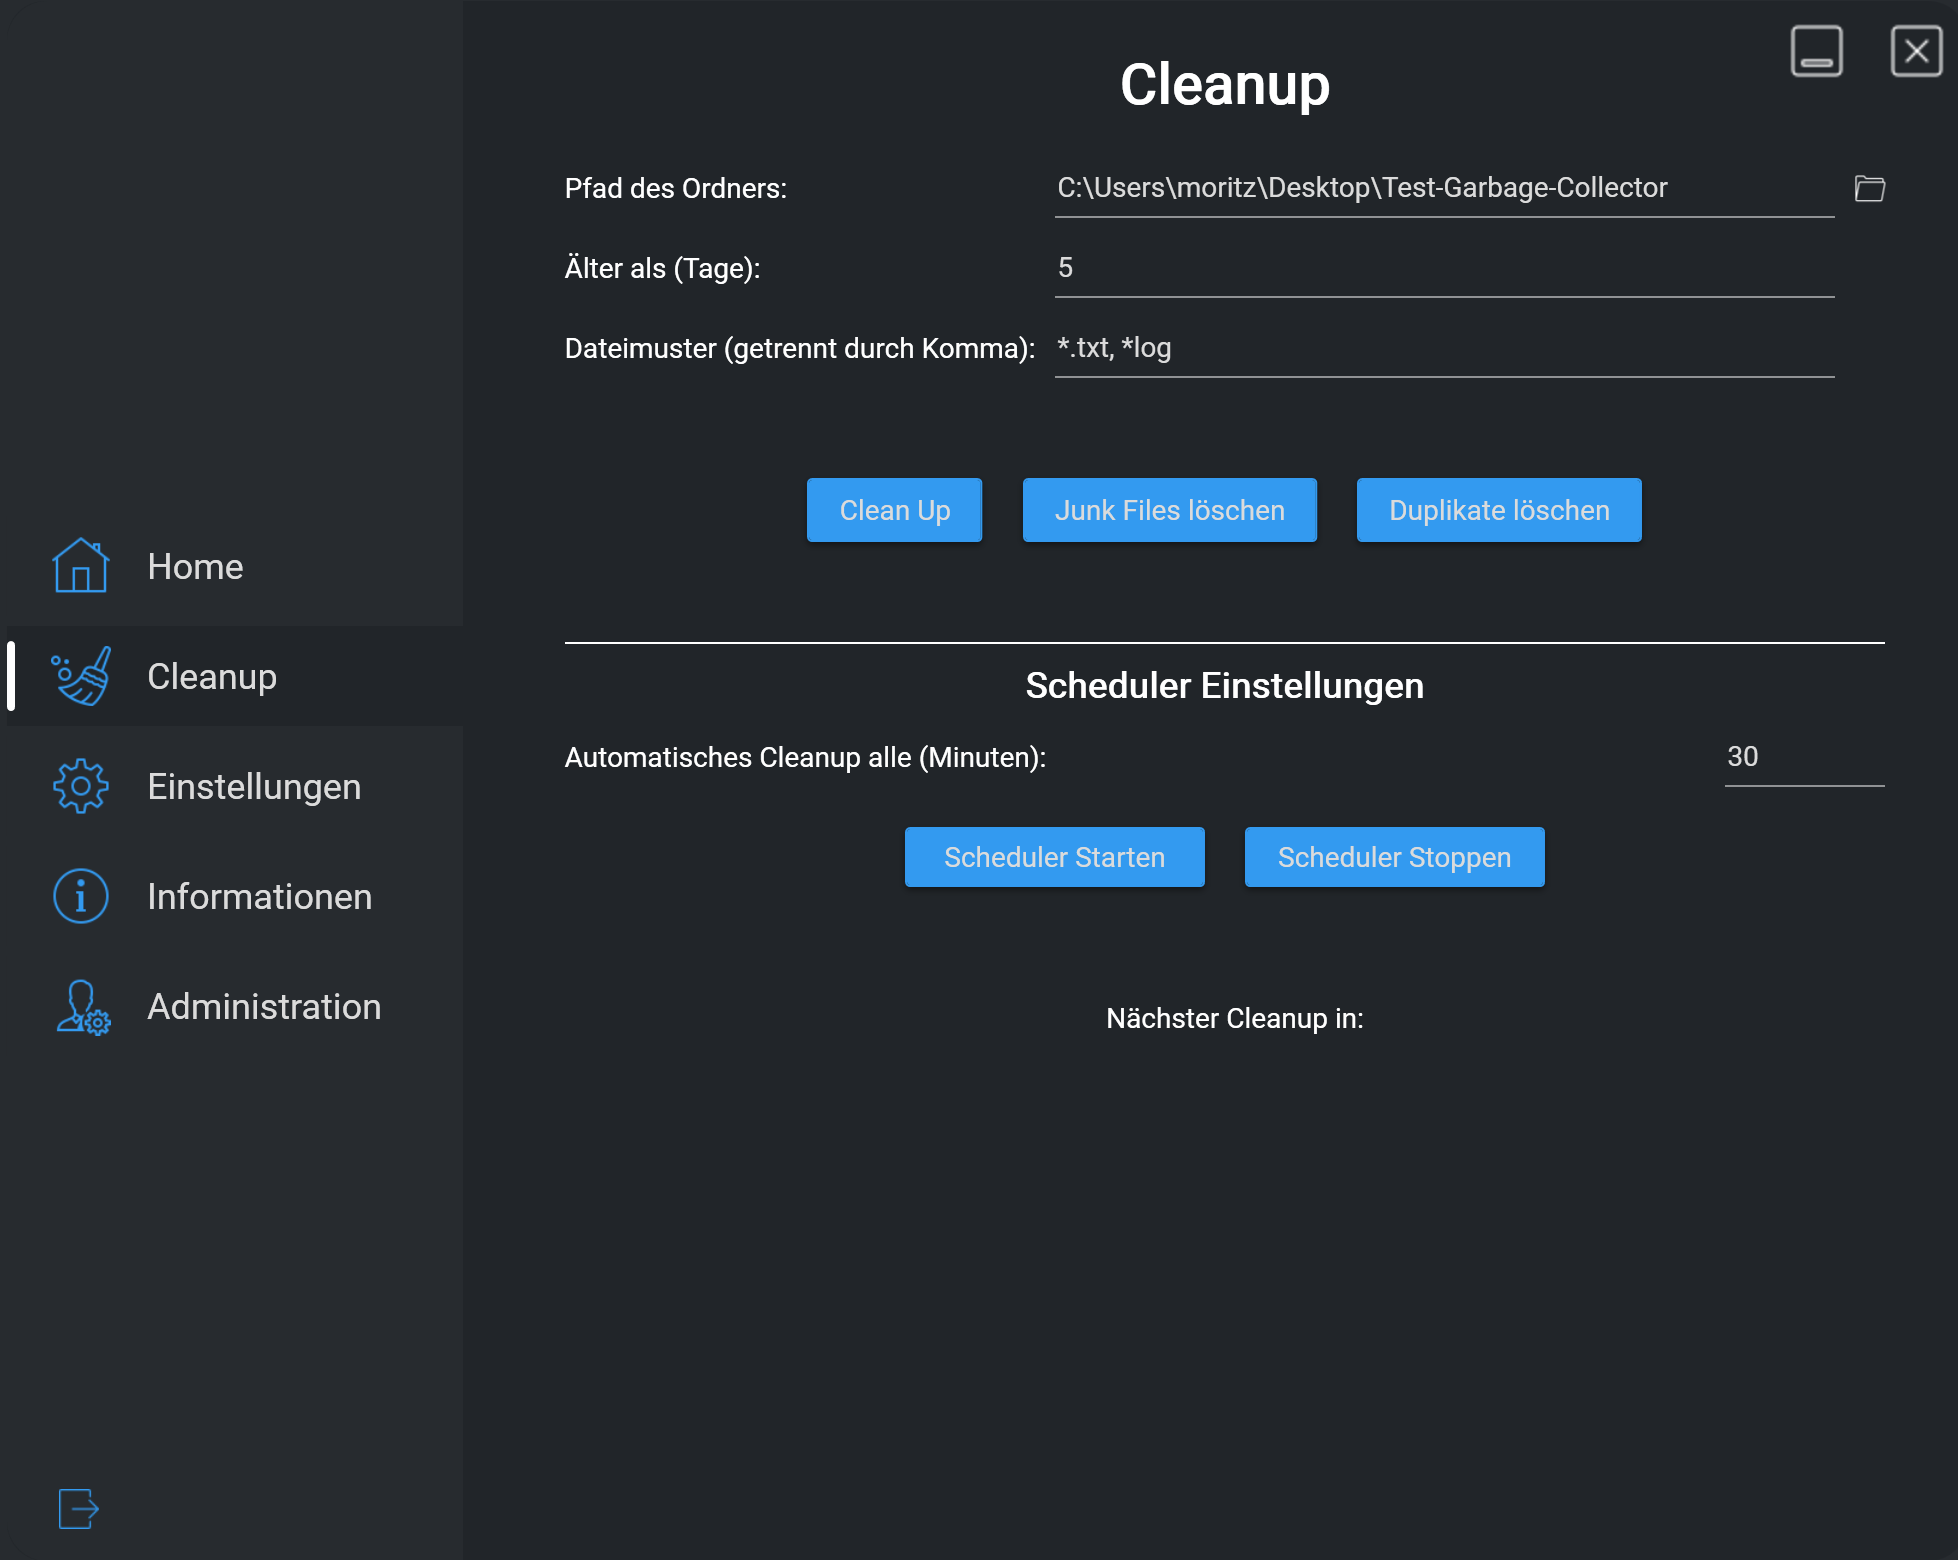
\includegraphics[width=0.9\textwidth]{src/screenshot_cleanup.png}
    \caption{Cleanup-Seite mit Optionen zur manuellen und automatischen Bereinigung}
\end{figure}

Im folgenden Screenshot ist die Bereinigungsfunktion inklusive laufendem Scheduler in Aktion zu sehen. Der Benutzer wird in Echtzeit über den Bereinigungsprozess informiert – inklusive Fortschrittsbalken und Anzeige der aktuell gelöschten Datei samt Pfadangabe. Während der Bereinigung sind alle Buttons deaktiviert (ausgegraut), um gleichzeitige Aktionen zu verhindern. Der Scheduler zeigt präzise an, wann der nächste automatische Cleanup durchgeführt wird.

\begin{figure}[H]
    \centering
    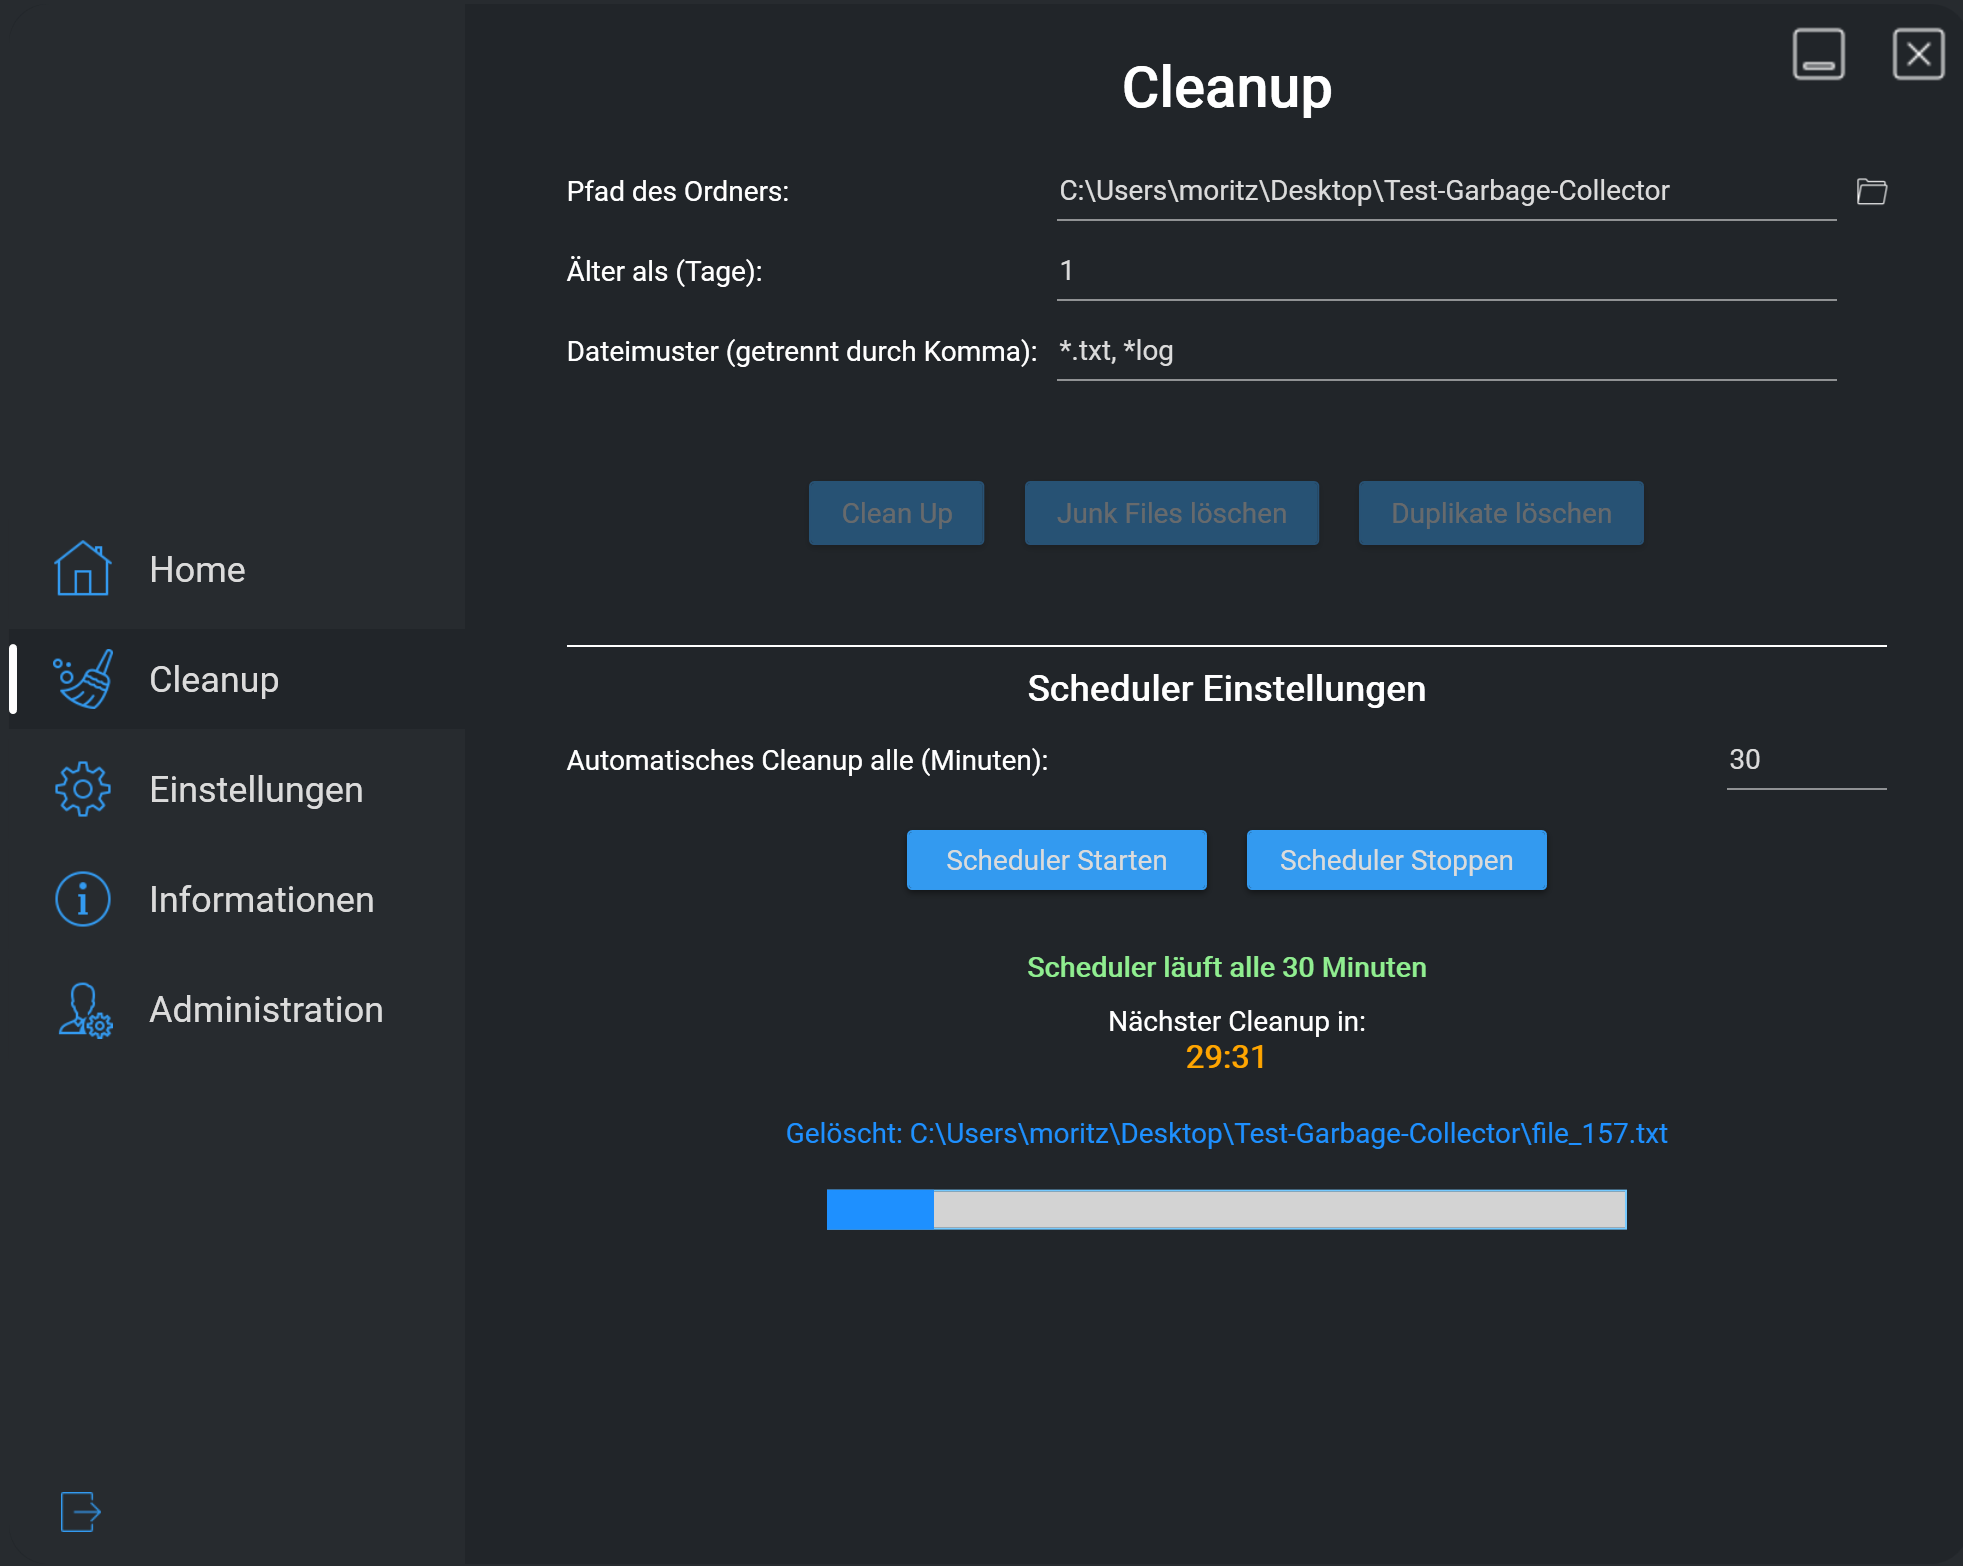
\includegraphics[width=0.9\textwidth]{src/screenshot_action.png}
    \caption{Cleanup-Seite mit laufendem Bereinigungsprozess und aktivem Scheduler}
\end{figure}

\vspace{1em}
Da es sich um ein konfigurationsdateigesteuertes Programm handelt, können die meisten Einstellungen auch direkt über eine Konfigurationsdatei (\texttt{config.json}) vorgenommen werden. Diese Datei wird beim ersten Start automatisch im Programmverzeichnis mit Beispieldaten angelegt und bleibt stets synchron mit den Einstellungen der Benutzeroberfläche.Auch der Connection String zur Datenbank lässt sich dort zentral anpassen. Details zur internen Handhabung und zur Konfiguration der Datenbankverbindung sind im Kapitel  \hyperref[sec:03_02_datenbankanbindung_und_docker]{\textbf{3.2 Datenbankanbindung und Docker}} erläutert.

\begin{figure}[H]
    \centering
    \begin{jsoncode}
{
  "SearchPath": "C:\\Users\\moritz\\Desktop\\Test-Garbage-Collector",
  "FilePatterns": [
    "*.txt"
  ],
  "OlderThanDays": 5,
  "DeleteDirectly": true,
  "DeleteRecursively": false,
  "ConnectionString": "Data Source=192.168.178.111;Initial Catalog=GarbageCollectorDB;"
}
\end{jsoncode}
    \caption{Beispiel einer möglichen \texttt{config.json}}
\end{figure}
% \begin{figure}[H]
%     \centering
%     \includegraphics[width=0.9\textwidth]{src/configjson_code.png}
%     \caption{Beispiel einer möglichen \texttt{config.json}}
% \end{figure}

